\section{Results}
\label{sec:results}

Figure~\ref{fig:layout} shows several different SRAM layouts
generated by OpenRAM in FreePDK45. OpenRAM can generate single
bank and multi-bank SRAM arrays. Banks are
symmetrically placed to have the same delay for data and address
while sharing peripheral blocks such as decoders.
\begin{figure}[tb]
\centering
\includegraphics[scale=.4]{./figs/layout.pdf}
\caption{Single bank and multi-bank SRAMs (not to scale) use
  symmetrical bank placement to share peripheral circuitry and
  equalize signal delays.}
\label{fig:layout}
\end{figure}

Figure~\ref{fig:density_figure} shows the memory area of different
total size and data word width memories in both FreePDK45 and
SCMOS. As expected, the smaller process technology (45nm) has lower
total area overall but the trends are similar in both technologies.

Figure~\ref{fig:density_figure} also shows the access time of
different size and data word width in FreePDK45 and SCMOS. Increasing
the memory size generally increases the access time; long bit-lines
and word-lines increase the access time by adding more parasitic
capacitance and resistance.  Since OpenRAM uses multiple banks and
column muxing, it is possible to have a smaller access time for larger
memory designs, but this will sacrifice density.

\begin{figure}[tb]
\begin{center}
\centering
%\includegraphics[width=8.5cm]{./figs/Results.pdf}
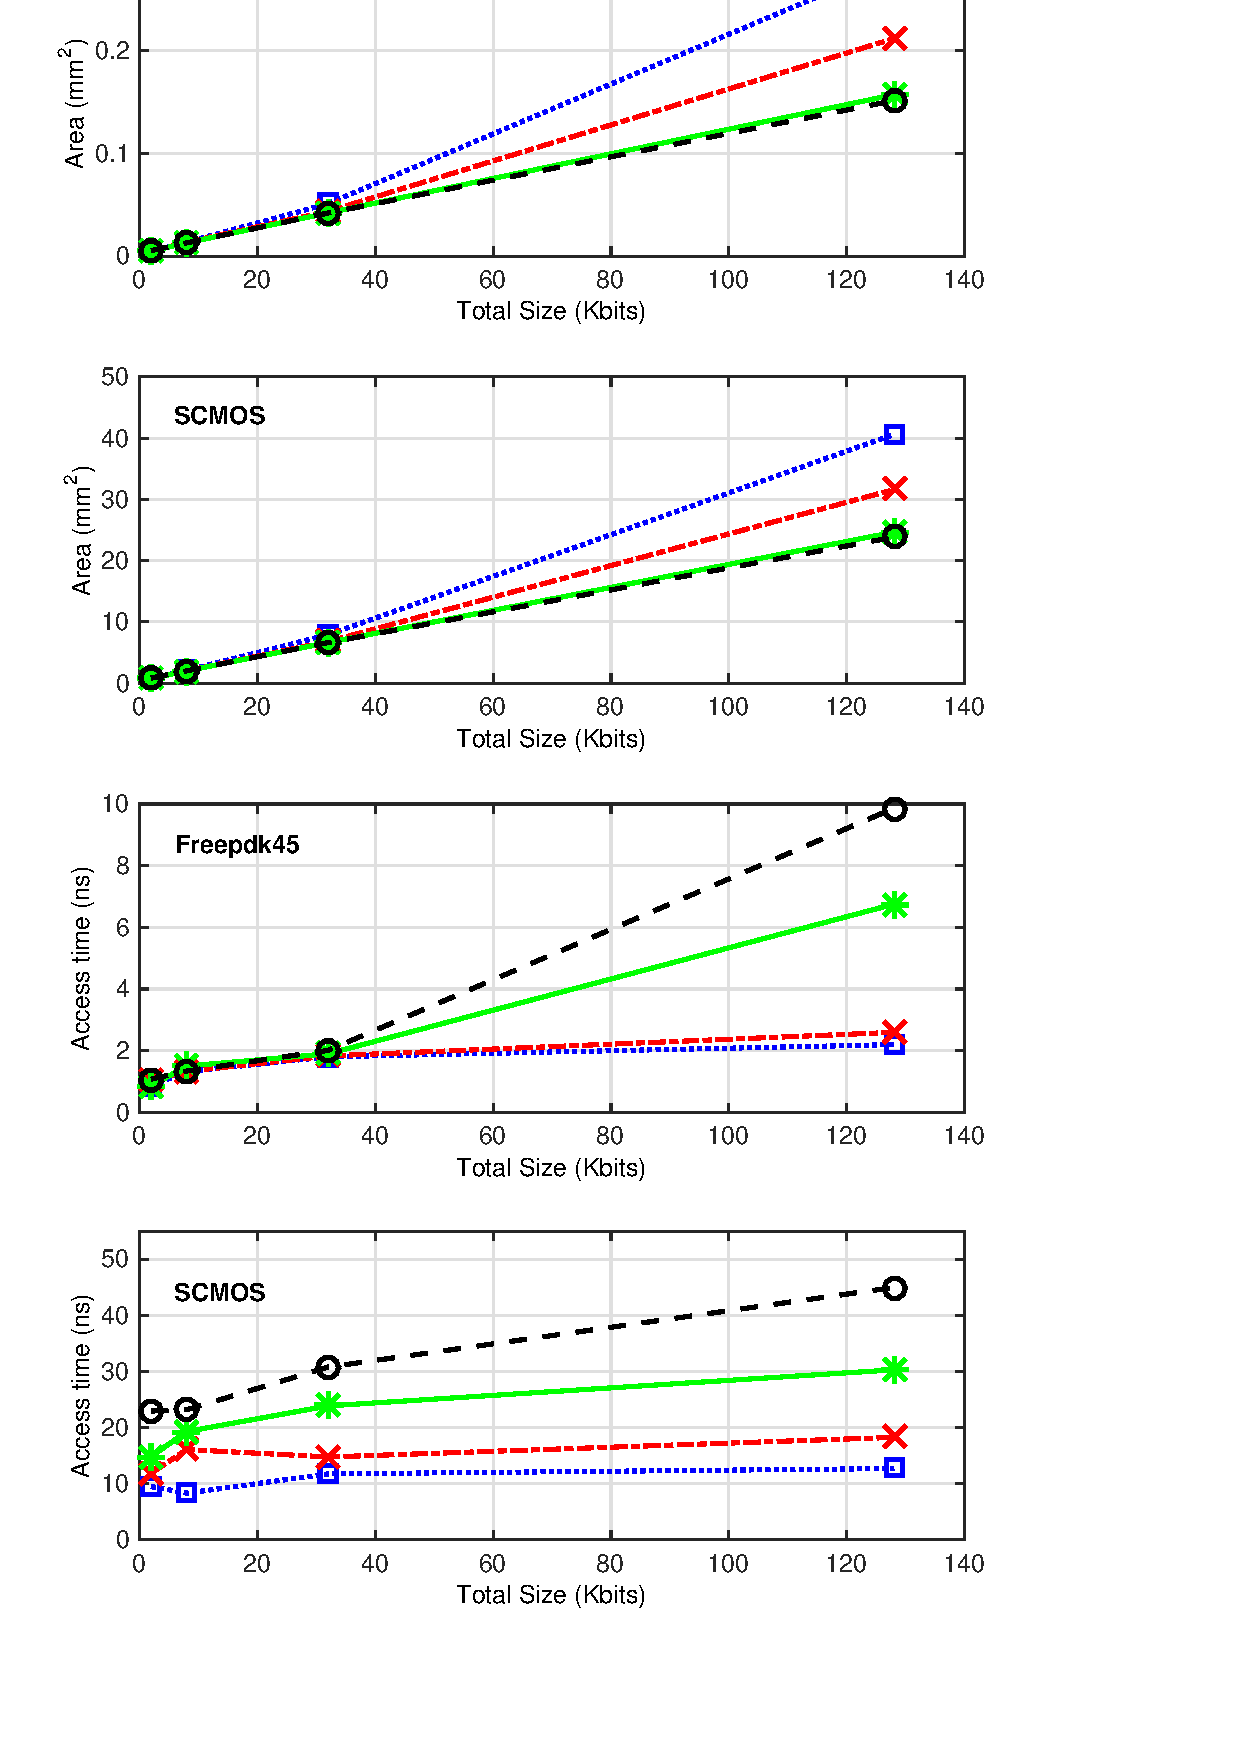
\includegraphics[width=7.5cm , height=14cm]{./figs/Results2.pdf}
%  \subfigure[FreePDK45 memory area \label{fig:freepdk_area}]{
%  \includegraphics[scale=1]{./figs/Freepdk_Area.pdf}}
%  \subfigure[SCMOS memory area \label{fig:scn3me_area}]{
%  \includegraphics[scale=.5]{./figs/Scn3me_Area.pdf}}
  \caption{OpenRAM provides high-density memories in multiple
    technologies and sizes with corresponding characterized
    delays. \label{fig:density_figure}}
  \vspace{-0.5cm}
\end{center}
\end{figure}

%Table~\ref{table:bit-density-comparison} shows a comparison between bit
%density of OpenRAM's generated memory designs and other publications
%which are close in technology node with FreePDK45 and SCMOS. As shown
%in this table, OpenRAM provides very dense SRAM arrays in both technologies.

\begin{table}[t]
\centering
\caption{OpenRAM has high density compared to other published memories in
  similar technologies.}
\begin{tabular}{|c|c|c|c|l|l|l|l|l|} \hline
\texttt{Ref.} & \texttt{Feature} & \texttt{Tech.} & \texttt{Density} \\
                   & \texttt{Size}    &               & [Mb/$mm^2$] \\
\hline \hline
$~\cite{4585946}$       & $65$ nm  & CMOS      & $0.7700$ \\ \hline
$~\cite{Bit_Density_3}$ & $45$ nm  & CMOS      & $0.3300$ \\ \hline
$~\cite{Bit_Density_2}$ & $40$ nm  & CMOS      & $0.9400$ \\ \hline
\verb+OpenRAM+          & $45$ nm  & FreePDK45 & $0.8260$ \\ \hline \hline
$~\cite{127339}$        & $0.5$ um & CMOS      & $0.0036$ \\ \hline
$~\cite{Bit_Density_6}$ & $0.5$ um & BiCMOS    & $0.0020$ \\ \hline
$~\cite{Bit_Density_5}$ & $0.5$ um & CMOS      & $0.0050$ \\ \hline
\verb+OpenRAM+          & $0.5$ um & SCMOS     & $0.0050$ \\ \hline
\end{tabular}
\label{table:bit-density-comparison}
\end{table}

%\begin{table*}
%\centering
%\caption{OpenRAM has high density, fast access time and low power consumption compared to other published memories in similar technologies.}
%\begin{tabular}{|c|l|l|l|l|l|l|l|l|} \hline
%\texttt{Reference} & \texttt{Technology} & \texttt{Density (Mb/$mm^2$)}& \texttt{Access time (ns)}& \texttt{Power consumption} \\ \hline \hline
%$~\cite{Bit_Density_1}$ & $65 nm CMOS$ & $0.77$ & $28$ & $22$ $uW/MHz$ \\ \hline
%$~\cite{Bit_Density_2}$ & $40 nm CMOS$ & $0.94$ & $45$ & $13.8$ $pJ/access/Mbit$ \\ \hline
%$OpenRAM$ & $45 nm FreePDK45$ & $0.826$ & $9.86$ & $13.14$ $mW$ \\ \hline \hline
%$~\cite{Bit_Density_4}$ & $0.5 um CMOS$ & $0.0036$ & $1.5$ & $6$ $W$ \\ \hline
%$~\cite{Bit_Density_6}$ & $0.5 um BiCMOS$ & $0.002$ & $1.5$ & $35$ $W$ \\ \hline
%$~\cite{Bit_Density_5}$ & $0.5 um CMOS$ & $0.005$ & $75$ & $3.9$ $mW$ \\ \hline
%$OpenRAM$ & $0.5 um SCMOS$ & $0.005$ & $44.9$ & $115$ $mW$ \\ \hline
%\end{tabular}
%\label{table:bit-density-comparison}
%\end{table*}

Comparison of power consumption and read access time of different
memories is a bit more complicated to make a conclusion, because there
are many trade-offs. Power and performance are highly dependent on
circuit style (CMOS, ECL, etc.), memory organization (more banks is
faster but sacrifices density), and the optimization goal: low-power
or high-performance.  In general, OpenRAM has reasonable trade-off
between the two and can be customized by using an alternate sense
amplifiers, decoders, or overall dimensional organization.
Table~\ref{table:bit-density-comparison} compares the bit-density of
OpenRAM against published designs using similar technology nodes. The
results show the benefit of technology scaling and that OpenRAM has
very good density in both technologies.  As a comparison, a 76ns SRAM
consumes 3.9mW~\cite{Bit_Density_5} while OpenRAM is much faster at
44.9ns but consumes 115mW for the same size. 

%Table~\ref{table:bit-density-comparison} shows a comparison between bit density, access
%time and power consumption of OpenRAM’s generated mem-
%ory designs and other publications which are close in tech-
%nology node with FreePDK45 and SCMOS. As shown in this
%table, OpenRAM provides very dense SRAM arrays in both
%technologies. There is no easy comparison on power con-
%sumption and read access time as these values vary with the
%array size and configuration. Therefore, we only try to com-
%pare the features of each work from a more general point of
%view.



